\documentclass[a4paper,11pt,french]{article}
\usepackage[utf8]{inputenc}

\usepackage[T1]{fontenc}
\usepackage[francais]{babel} 
\usepackage[top=2cm, bottom=2cm, left=2cm, right=2cm, includeheadfoot]{geometry} %pour les marges
\usepackage{lmodern}
\usepackage{pict2e}
\usepackage{tikz}	
\usepackage{tikz-uml}
\usepackage{fancyhdr} % Required for custom headers
\usepackage{lastpage} % Required to determine the last page for the footer
\usepackage{extramarks} % Required for headers and footers
\usepackage{graphicx} % Required to insert images
\usepackage{tabularx, longtable}
\usepackage{color, colortbl}
\usepackage{lscape}
%\usepackage[hidelinks]{hyperref}
\usepackage{longtable}
\usepackage{multirow}
\usepackage{rotating}
\usepackage{gensymb}

\usepgflibrary{arrows} % for pgf-umlsd

\usetikzlibrary{trees,shapes.geometric,arrows,decorations.pathmorphing,backgrounds,fit,positioning,shapes.symbols,chains	}

\linespread{1.1} % Line spacing

% Set up the header and footer
\pagestyle{fancy}
\lhead{\textbf{\hmwkClass -- \hmwkSubject \\ \hmwkTitle \\ \hmwkDocName}} % Top left header
\rhead{
\includegraphics[width=10em]{./pics/logo_univ.png}}
\lfoot{\lastxmark} % Bottom left footer
\cfoot{} % Bottom center footer
\rfoot{Page\ \thepage\ / \pageref{LastPage}} % Bottom right footer
\renewcommand\headrulewidth{0.4pt} % Size of the header rule
\renewcommand\footrulewidth{0.4pt} % Size of the footer rule

\setlength{\headheight}{40pt}

\newcommand{\hmwkTitle}{Transchiffrement} % Assignment title
\newcommand{\hmwkClass}{Master 2 SSI } % Course/class
\newcommand{\hmwkAuthorName}{Yves Nouafo} % Your name
\newcommand{\hmwkSubject}{Conduite de projet} % Subject
\newcommand{\hmwkDocName}{État de l'art sur les collisons MD5} % Document name

\newcommand{\version}{1.0} % Document version
\newcommand{\docDate}{2 Janvier 2014} % Document date
\newcommand{\checked}{} % Checker name
\newcommand{\approved}{Magali Bardet} % Approver name

\makeatletter
\newcommand{\resettranslate}{\let\translate\@firstofone}
\makeatother

\definecolor{gris}{rgb}{0.95, 0.95, 0.95}

\title{
\vspace{2in}
\textmd{\textbf{\hmwkClass :\ \hmwkTitle}}\\
\normalsize\vspace{0.1in}\small{Due\ on\ \hmwkDueDate}\\
\vspace{0.1in}\large{\textit{\hmwkClassInstructor\ \hmwkClassTime}}
\vspace{3in}
}

\author{\hmwkAuthorName}
\date{} % Insert date here if you want it to appear below your name


\usepackage{amsmath}
\begin{document}
\newcount\startdate
\newcount\daynum
%\pgfcalendardatetojulian{2013-01-021}{\startdate}
\pagestyle{fancy}

\vspace*{5cm}
\begin{center}\textbf{\Huge{\hmwkDocName}}\end{center}
\vspace*{4.5cm}
	

\fcolorbox{black}{gris}{
\begin{minipage}{15cm}
\begin{tabularx}{10cm}{lXl}
	\bfseries{Version} & & \version\\
	& & \\
	\bfseries{Date} & & \docDate\\
	& & \\
	\bfseries{Rédigé par} & & \hmwkAuthorName \\
	& & \\
	\bfseries{Relu par} & & \checked \\
	& & \\
	\bfseries{Approuvé par} & & \approved \\
	& & \\
\end{tabularx}
\end{minipage}
}

\newpage

%Tableau de mises à jour
\vspace*{1cm}
\begin{center}
\textbf{\huge{MISES À JOUR}}\\
\vspace*{3cm}
	\begin{tabularx}{16cm}{|c|c|X|}
	\hline
	\bfseries{Version} & \bfseries{Date} & \bfseries{Modifications réalisées}\\
	\hline
	1.0 & 02/01/2014 & Création\\
	\hline
	& & \\
	\hline
	\end{tabularx}
\end{center}

%La table des matières
\clearpage
\tableofcontents
\clearpage

%%==========================================================================
%%==========================================================================
\section{Introduction}
La sécurité informatique est un axe important dans le monde de l'informatique. Ces dernières années, on peut constater que plusieurs méthodes de cryptographie ont été développées. Ces méthodes reposent sur les fonctions de hachage cryptographique. Ce sont des fonctions qui associent à un message de longueur arbitraire une chaine d'octets de longueur fixe appelé {\it{hashé}}.\\

Les fonctions de hachage doivent satisfaire les principes suivant:
\begin{itemize}
  \item résistante au calcul de collision
  \item résistante au calcul de seconde pre-image
  \item résistante au calcul de pré-image
\end{itemize}
\vspace{.5cm}

Une des fonctions de hachage les plus utilisés est MD5, inventé par Rivest en 1992. MD5 comme toute fonctions de hachage elle prend en entrée un message de longueur variable et retourne une chaine de longueur fixe, soit 128 bits.\\

Le but de cette étude est de décrire le fonctionnement interne de la fonction de hachage MD5 et d'en réaliser un état de l'art sur sa résistance aux collisions. Plus précisément, comment générer des entrées différentes pour la fonction MD5 de telle sorte que ces deux entrées aient le même hashé MD5.\\
Nous verrons ensuite quel(s) impact(s) une collision sur des certificats peut avoir, notamment lorsque celui-ci est appliqué au transchiffrement.

%%==========================================================================
%%==========================================================================
\section{Le schéma de Merkle-Damgard}
Le schéma de merkle-Damgard décrit comment construire une fonction de hachage munie d'une fonction de compression. MD5 est basé sur ce schéma dont le principe de fonctionnement est le suivant:\\

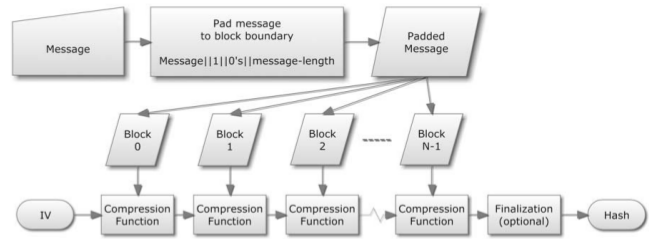
\includegraphics[scale=.61]{./pics/md.png}
\vspace{.5cm}

\begin{itemize}
\item La fonction de compression prend en entrée un bloc B de taille 512 bits et une IHV (valeur de hachage intermmédiaire) de 128 bits.
\item Chaque messages passés en paramètre doit subir un padding si sa taille n'est pas multiple de 512 bits.
\item Le message est ensuite découpé en N blocks de 512 bits.
\item La fonction de hachage commence avec une IHV initial appelé {\it{IV}}.
\item Chaque blocs de message $M_{i}$ est appelé avec la valeur courante $IHV_{i}$ et la fonction de compression calcul une nouvelle valeur $IHV_{i+1}$. Lorsque tout les blocs sont traités le {\it{hashé}} final $IHV_{N}$ est construit.
\end{itemize}
\vspace{.5cm}

%%==========================================================================
%%==========================================================================
\section{Fonctionnement de MD5}
MD5 fonctionne de la manière suivante:\\
\begin{enumerate}
\item {\it{\bf{le padding}}}. On ajoute un pad au message initial si sa longueur n'est pas un multiple de 512 bits. Le padding consiste à ajouter une séquence de bits dont le premier bit est à 1 suivi de 0 de telle sorte que la longueur résultante soit égale à 448 mod 512. Les bits restants sont utilisés pour ajouter la longueur du message initial ;
\item {\it{\bf{le partitionnement}}}. MD5 découpe le message original (avec un padding ou non) en N blocs $M_{i}$, ..., $M_{N}$ de 512 bits ;
\item {\it{\bf{le processus}}}. MD5 calcule des valeurs intermémdiaire de hash, {\it{IHV}}.
  \begin{itemize}
  \item Chaque IHV est diviser en 4 mots de 32 bits (a, b, c, d).
  \item L'{\it{IV}} initial est ($a_{0}$, $b_{0}$, $c_{0}$, $d_{0}$) = ($67452301_{16}$, $EFCDAB89_{16}$, $98BADCFE_{16}$, $10325476_{16}$).
  \item Chaque IHV calculée en utilisant la fonction de compression MD5Compress telle que:\\ $IHV_{i}$ = MD5Compress($IHV_{i-1}$, $M_{i}$) ;
  \end{itemize}
\item {\it{\bf{le résultat}}}. Le {\it{hashé}} produit est la concaténation en hexadécimal des dernières valeurs\\ (a, b, c, d) calculés.
\end{enumerate}

%%==========================================================================
%%==========================================================================
\section{La fonction de compression de MD5}
La fonction de compression de MD5 prend en paramère une IHV de 128 bits et un bloc de message de 512 bits. Elle s'effectue en 64 étapes découpés en 16 tours. À chaque étape les opérations suivantes sont réalisés:\\

%%==========================================================================
\subsection{Les opérations internes}
\begin{enumerate}
\item {\bf{l'addition et sa constante AC}}:\\
$AC_{t}$ = 2\up{32}|sin(t + 1)| \hspace{.5cm} pour 0 <= t <= 64\\

\item \bf{la rotation gauche et ses constantes RC}:\\
($RC_{t}$, $RC_{t+1}$, $RC_{t+2}$, $RC_{t+3}$) =
$\left\{
\begin{array}{l}
  (7, 12, 17, 22)   \hspace{.8cm}pour \hspace{.2cm} t = 0, 4, 8, 12 \\
  (5, 9, 14, 20)  \hspace{1cm}pour \hspace{.2cm} t = 16, 20, 24, 28 \\
  (4, 11, 16, 23)  \hspace{.8cm}pour \hspace{.2cm} t = 32, 36, 40, 44 \\
  (6, 10, 15, 21)  \hspace{.8cm}pour \hspace{.2cm} t = 48, 52, 56, 60 \\
\end{array}
\right.$
\vspace{.5cm}
\item \bf{une fonction non-linéaire $f_{t}$}:\\

$f_{t}$(x, y, z) =
$\left\{
\begin{array}{l}
  F(x, y, z) = (x  \bigwedge y) \bigoplus (\bar x \bigwedge z) \hspace{1.128cm} 0 <= t < 16\\
  G(x, y, z) = (z  \bigwedge x) \bigoplus (\bar z \bigwedge y) \hspace{.97cm} 16 <= t < 32\\
  H(x, y, z) = x \bigoplus y \bigoplus z \hspace{2cm} 32 <= t < 48\\
  I(x, y, z) = y \bigoplus (x \bigvee \bar z) \hspace{2cm} 48 <= t < 64\\
\end{array}
\right.$
\vspace{.5cm}
\end{enumerate}

%%==========================================================================
\subsection{Traitement des blocs de message}
les blocs de message sont découpés en 16 mots consécutif $M_{0}$, ..., $M_{15}$. Les blocs de mots sont ensuite étendu à 64 mots $W_{t}$ pour 0 <= t <= 64 de 32 bits chacun telle que:
\vspace{.5cm}

$W_{t}$ =
$\left\{
\begin{array}{l}
  m_{t} \hspace{2.8cm} 0 <= t < 16\\
  m_{(1 + 5t) mod 16} \hspace{1cm} 16 <= t < 32\\
  m_{(5 + 3t) mod 16} \hspace{1cm} 32 <= t < 48\\
  m_{(7t) mod 16} \hspace{1.4cm} 48 <= t < 64\\
\end{array}
\right.$
\vspace{.5cm}

%%==========================================================================
\subsection{État interne de la fonction de compresion}
Lors de chaque appel de la fonction de compression de MD5, son état interne est sauvegarder. L'état interne n'est autre que les mots $m_{t}$ vu dans la section précédente. Chaque mot est sauvegardé dans un registre Q = {$Q_{t}$, $Q_{t-1}$, $Q_{t-2}$, $Q_{t-3}$}. Le nouvel état $Q_{t+1}$ est calculé en initialisant ($Q_{t}$, $Q_{t-1}$, $Q_{t-2}$, $Q_{t-3}$) = (b, c, d, a) pour {\it{t}} = 0, 1, ..., 63, $Q_{t}$ et calculé comme suit:
\vspace{.5cm}

$\left\{
\begin{array}{l}
  F_t = f_t(Q_t, Q_{t-1}, Q_{t-2}) \\
  T_t = F_t + Q_{t-3} + AC_t + W_t \\
  R_t = RL(T_t, RC_t) \\
  Q_{t+1} = Q_t + R_t \\
\end{array}
\right.$
\vspace{.5cm}

Lorsque toutes les étapes de caluls sont finies l'état des mots finaux sont ajoutés à l'IHV et la fonction retourne comme valeur MD5Compress(IHV, B) = (a + $Q_{61}$, b + $Q_{64}$, c + $Q_{63}$, d + $Q_{62}$).

%%==========================================================================
\subsection{L'algorithme de fonction de compression}
L'algorithme de fonction de collision est réalisé de la manière suivante:\\

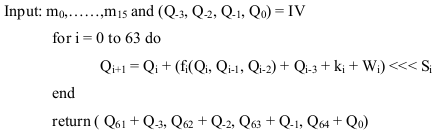
\includegraphics[scale=.61]{./pics/algocom.png}

%%==========================================================================
\subsection{Schématisation du fonctionnement de MD5}
Le fonction de MD5 est montré par le schéma suivant, où $CV_{q}$ est l'ensemble des chaines IHV, $Y_{q}$ est q\up{ième} bloc de message de longueur 512 bits.\\

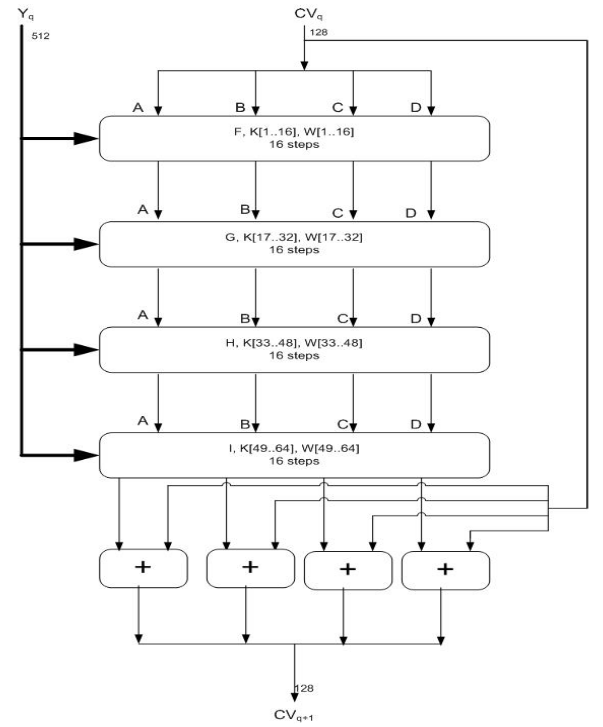
\includegraphics[scale=.61]{./pics/md5process.png}

%%==========================================================================
%%==========================================================================
\section{Étude de failles sur MD5}

Les premières collisions ont été trouvées par les équipes de Wang et Yu en 2004. Leur procédé s'appuie sur la cryptananlyse de la fonction de compression de la fonction de hachage de MD5. 

Leur technique consistait à trouver des collisions en éxecutant une seule fois la fonction de hachage MD5 en analysant les changements effectués sur les bits à chaque tours.

%%==========================================================================
\subsection{Présentation de l'attaque menée par Wang et Yu}
L'attaque proposé par Wang et Yu consistait à trouver un couple de message (M, M') qui ont un même hashé MD5. De manière plus précise on a:
\begin{itemize}
  \item M = ($M_{0}$, $M_{1}$)
  \item M' = ($M'_{0}$, $M'_{1}$)
\end{itemize}
où chaque $M_{i}$ et $M'_{i}$ est un bloc de 512 bits ayant chacun 16 mots de 32 bits.

La méthode utilisée par Wang et Yu est une attaque différentielle.


%M\subsubsection{Cryptanalyse différentielle}
%Wang et Yu utilise comme entrée pour la fonction MD5 la différence modulaire (soustraction en les bits modulo 2\up{32} des messages).\\

%//////


\subsubsection{Attaque différentielle sur MD5 menée par Wang et Yu}
On considère que pour le message M, l'IV initial de MD5 est IV = (a, b, c, d) et que le vecteur du second bloc est $IV_{1}$ = ($a_{1}$, $b_{1}$, $c_{1}$, $d_{1}$) = ($Q_{61}$, $Q_{64}$, $Q_{63}$, $Q_{62}$) + (a, b, c, d) et où ($Q_{61}$, $Q_{64}$, $Q_{63}$, $Q_{62}$) = $MD5_{1..64}$(IV, $M_{0}$) et la valeur hashé h est h = $MD5_{1..64}$($IV_{1}$, $M_{1}$) + ($a_{1}$, $b_{1}$, $c_{1}$, $d_{1}$). De la même manière on va définir les valeurs $IV'_{1}$ et h' pour les messages $M'_{0}$ et $M'_{1}$ de M'.\\

La différence modulaire passée en entrée de la fonction MD5 doit respecter les conditions suivante:
\begin{itemize}
\item (delta)$M_{0}$ = $M'_{0}$ - $M_{0}$ = (0, 0, 0, 0, 2\up{31}, 0, 0, 0, 0, 0, 0, 2\up{15}, 0, 0, 2\up{31}, 0)
\item (delta)$M_{1}$ = $M'_{1}$ - $M_{1}$ = (0, 0, 0, 0, 2\up{31}, 0, 0, 0, 0, 0, 0, -2\up{15}, 0, 0, 2\up{31}, 0)
\item (delta)$IV_{1}$ = $IV'_{1}$ - $IV_{1}$ = (2\up{31}, 2\up{25} + 2\up{31}, 2\up{25} + 2\up{31},2\up{25} + 2\up{31})
\item (delta)h = h' - h = (0, 0, 0, 0)
\end{itemize}
\vspace{.5cm}
La différence des mots entre $M'_{0}$ et $M_{0}$ et entre $M'_{1}$ et $M_{1}$ s'effectue tous deux aux mots 4, 11 et 14.\\


\subsubsection{Algorithme de l'attaque menée par Wang et Yu}
\begin{enumerate}
 \item Générer un bloc de message $M_0$ de 512 bits.
 \item Réaliser les opérations pour chaque étape et modifier $M_0$ en s'assurant que toutes les conditions sur les variables soient satisfaite. Dans le cas contraire, recommencer.
 \item Vérifier que les différences requises soient satisfaite et dans ce cas nous avons trouver un message $M_0$ nécessaire pour l'attaque.
 \item Utiliser la sortie MD5 après avoir traiter $M_0$ pour initialiser les valeur de $M_1$.
 \item Après avoir trouvé $M_0$, générer le bloc de message $M_1$ de 512 bits.
 \item Réaliser les opérations pour chaque étape et modifier $M_1$ en s'assurant que toutes les conditions sur les variables soient satisfaite. Dans le cas contraire, recommencer.
 \item Vérifier que les différences requises soient satisfaite et dans ce cas nous avons trouver un message $M_1$ nécessaire pour l'attaque.
 \item Vérifier que les différences requises soient satisfaite et dans ce cas nous avons trouver une collision.
 \item Calculer $M'_0$ = $M_0$ + (delta)$M_0$ et $M'_1$ = $M_1$ + (delta)$M_1$
 \item MD5(M) = MD5(M').
\end{enumerate}

L'algorithme présenté implante la méthode menée par Wang et Yu.Elle recherche les blocs 1 et 2 de messages pour trouver une collision. Les messages générer sont construit dans un fichier crée.

%%==========================================================================
\subsection{Présentation de l'attaque menée par Marc Stevens}
Marc Stevens reprend les travaux réalisés par Wang et Yu et améliore leurs algorithmes en y introduisant de nouvelles notions et montre comment à partir de deux messages arbitraires, il est possible de générer des collisions sous MD5.\\

La différence technique entre ces deux travaux repose sur le fait que pour créer une collision, Stevens utilise un seul bloc de collision au lieu de deux comme le faisait Wang et Yu. 

\subsubsection{Attaque à préfixes choisis}
Tout comme la méthode utiliser par Wang et Yu, les deux messages initiaux peuvent avoir des longueur différentes. Dans ce cas, il faut appliquer un padding au plus court des deux, pour qu'elles aient des longueurs égales. En agissant de la sorte, lorsque les message seront passé à la fonction de compression de MD5, on s'assure que qu'ils auront le même padding.

La technique repose sur le fait qu'on peut trouver un couple de message de longueur k-bits tel que, concatener au dernier bloc de message incomplet, on trouve une différence entre les IHVs après application de la fonction de compression de MD5 au couple de message étendu. Ces k-bits sont calculés grace eu théorème des anniversaires.

L'idée principale est d'éliminer la difference (delta)IHV en r étape où r désigne les étapes pour construire r bloc de quasi collisions.

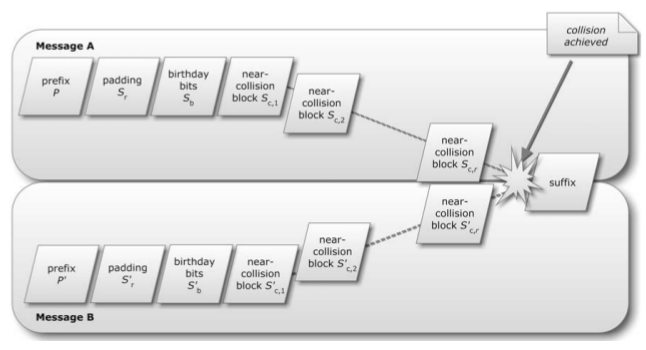
\includegraphics[scale=.61]{./pics/col.png}


\subsubsection{Construction des préfixes choisis de collisions}
Un préfixe choisi de collision est un couple de messages (M, M') qui consiste à choisir arbitrairement des préfixes P et P', construit avec des suffixes S et S' de telle sorte que l'on ait:\\
M = P || S et M' = P' || S' et MD5(M) = MD5(M').\\

Les suffixes S et S' ont la même structure. Ils sont découpés en 3 parties.
\begin{itemize}
\item le padding $S_{r}$. $S_{r}$ est choisi telle que P || $S_{r}$ || $S_{b}$ où P' || $S'_{r}$ || $S'_{b}$ soit multiple de 512 ;
\item les bits d'anniversaire $S_{b}$. Ils sont choisit de façon à respecter certaine condition (chemin différentiel) et servent à réduire le nombre d'appel de la fonction de commpression de MD5 pour parvenir à trouver une collision. En introduisant cette chaine de bits on parvient ainsi d'un nombre d'appel de 2\up{59} à 2\up{39}. Ce qui reste largement en dessous du temps limite de calcul que l'on peut faire de nos jours ;
\item bit de quasi-collision $S_{c}$. Utiliser pour éliminer la différence (delta) $IHV_N$ = $IHV_N$ - $IHV'_N$ où $IHV_N$ (resp. $IHV'_N$) est le résultat IHV renvoyé par la fonction MD5Compress appliqué au message P || $S_{r}$ || $S_{b}$ (resp. P' || $S'_{r}$ || $S'_{b}$) .
\end{itemize}
\vspace{.5cm}


\subsubsection{Chemin différentiel et bits de condition}
Nous avons vu en section 4.3 l'état interne lors d'un appel de la fonction de compression de MD5. Si on applique MD5Compress aux entrées (IHV, B) et (IHV', B') le chemin différentiel de la fonction MD5Compress est définie de la fa\c on suivante.\\

$\left\{
\begin{array}{l}
  (delta)F_t = f_t(Q'_t, Q'_{t-1}, Q'_{t-2}) - f_t(Q_t, Q_{t-1}, Q_{t-2}) \\
  (delta)T_t = (delta)F_t + (delta)Q_{t-3} + (delta)W_t \\
  (delta)R_t = RL(T'_t, RC_t) - RL(T_t, RC_t) \\
  (delta)Q_{t+1} = (delat)Q_t + (delta)R_t \\
\end{array}
\right.$
\vspace{.5cm}

La propagation du chemin diiférentiel se fait à travers les 64 étapes de la fonction MD5 et est issue de (delta)IHV et (delta)B.

\subsubsection{Les bits de conditions}
Le chemin différentiel est calculé à l'aide de bits de conditions à un état t du mots sauvegardé par la fonction de compression de MD5. En d'autres termes, le chemin différentiel est calculé sur $Q_t$ et $Q'_t$ où un bit de condition peut être calculé de manière direct ou indirect à partir des valeurs de bits de $Q_t$[i] et $Q'_t$[i]. Le chemin différentiel est alors une matrice de 68 lignes (-3 <= t <= 64) et 32 colonnes pour chaque bits.\\

Un bit de condition direct sur un état Q ou Q' ne doit pas modifier d'autres bits de cet état Q où Q'. Un bit de condition direct par contre peut modifier l'etat d'un bit de Q ou Q'. Les bits de conditions sont données comme suit:\\


\begin{tabular}{lll}
\hline
	$Q_t$[i] &\vline \hspace{.1cm} Condition sur ($Q_t$[i], $Q'_t$[i]) &\vline \hspace{.1cm} $k_i$ \\ \hline
	. &\vline \hspace{.1cm} $Q_t$[i] = $Q'_t$[i] &\vline \hspace{.1cm} 0 \\ \hline
	+ &\vline \hspace{.1cm} $Q_t$[i] = 0, $Q'_t$[i] = 1 &\vline \hspace{.1cm} +1 \\ \hline
	- &\vline \hspace{.1cm} $Q_t$[i] = 1, $Q'_t$[i] = 0 &\vline \hspace{.1cm} -1 \\ \hline
\end{tabular}

\subsubsection{Construction du chemin différentiel}
la construction du chemin différentiel est définit par l'algorithme suivant: 
\begin{itemize}
  \item Utiliser IHV et IHV' qui détermine les bits de condition ($q_i$) -3 <= i <= 0
  \item Construire un chemin différentiel partiel dit faible pour les étapes 0 ... 11 de la fonction de hachage MD5 en étendant les $q_i$.
  \item La construction d'un chemin différentiel partiel dit fort pour les étapes 16 ... 63 de la fonction de hachage MD5 en étendant les $q_i$.
    \item essayer de connecter les deux chemins différentiels aux étapes 12 ... 15. Si ce n'est pas possible, rechercher d'autre chemin différentiel dit fort et faible qui remplisse les conditions.
\end{itemize}

%%==========================================================================
\subsection{Complexité des attaques sur MD5}

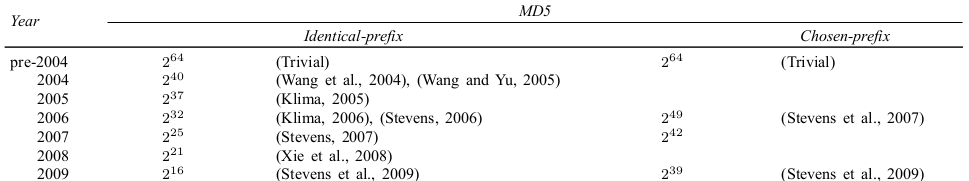
\includegraphics[scale=.50]{./pics/complexite.png}

\vspace{.5cm}
Au cours du temps les méthodes de cryptanalyse utilisant les résulats des recherches de Wang et Yu sur MD5 ont été amélioré. 

///

%%==========================================================================
%%==========================================================================
\section{Application d'exploitation de collision MD5}

L'état de l'art de la collision MD5 faite dans les chapitres précédents peut être appliqué dans la vie réelle. On peut citer par exemple, la collision entre documents, la vérification de l'intégrité d'un logiciel ou encore, en ce qui nous concerne, la création de faux certificats d'autorité. \\

Dans ce chapitre, nous allons voir comment comment construire construire deux certificats X.509 avec des noms distinctifs mais ayant les mêmes signature électronique.

%%==========================================================================
\subsection{Rappel sur les certificats X.509}

X.509 est une norme de cryptographie de l'Union internationale des télécommunications pour les infrastructures à clés publiques (PKI). Il établit entre autres les formats standard de certificats électroniques et un algorithme pour la validation de chemin de certification. X.509 à été crée en 1988  et repose sur un système hiérarchique d'autorités de certification, à l'inverse des réseaux de confiance (comme PGP), où n'importe qui peut signer (et donc valider) les certificats des autres.\\

Dans le système X.509, une autorité de certification attribue un certificat liant une clé publique à un nom distinctif (Distinguished Name), à une adresse électronique ou un enregistrement DNS.\\

Les certificats racines sont des clés publiques non signées, ou auto-signées, dans lesquels repose la confiance. Des autorités de certification commerciales détiennent des certificats racines présents dans de nombreux logiciels, par exemple les navigateurs Web. Quand le navigateur ouvre une connexion sécurisée (SSL) vers un site ayant acheté une certification auprès d'une autorité connue, il considère le site comme sûr dans la mesure où le chemin de certification est validé. Le passage en mode sécurisé est alors transparent.\\

Si le certificat est auto-signé (autorité de certification et créateur de la clé publique ne font qu'un), le navigateur propose de l'examiner, puis de l'accepter ou de le refuser selon la confiance qu'on lui accorde.\\

%%==========================================================================
\subsection{Structure d'un certificat}

\begin{itemize}
\item Version
\item Numéro de série
\item Algorithme de signature du certificat
\item Nom du signataire du certificat
\item Validité (dates limite) 
  \begin{itemize} 
  \item Pas avant
  \item Pas après
  \end{itemize}
\item Détenteur du certificat
\item Informations sur la clé publique :
  \begin{itemize}
  \item Algorithme de la clé publique
  \item Clé publique proprement dite
  \end{itemize}
\item Identifiant unique du signataire (optionnel, à partir de X.509 version 2)
\item Identifiant unique du détenteur du certificat (optionnel, à partir de X.509 version 2)
\item Extensions (optionnel, à partir de X.509 version 3)
  \begin{itemize}
  \item Liste des extensions
  \end{itemize}
\end{itemize}

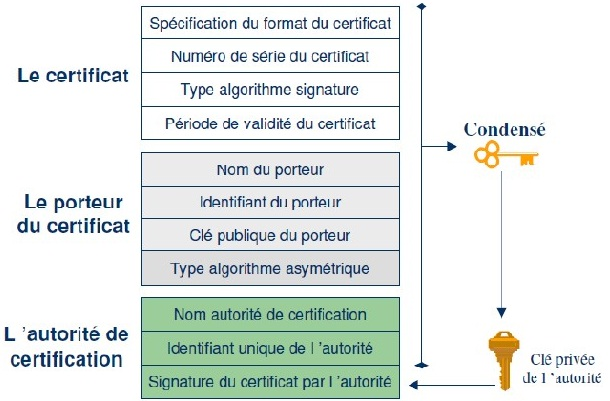
\includegraphics[scale=.61]{./pics/cert.jpg}

%%==========================================================================
\subsection{Création d'un faux certificat}
Lorsque l'on génère deux certificats X.509 qui ont des signatures identiques mais des Distinguish Name différent on intervient directement sur le module RSA (la clé publique).\\

Nous avons vu que pour générer une collision à préfixe choisi, il faut calculer des préfixes qui permette de calculer des collisions. En application sur les certificats, le préfixe du vrai certificat contient le DN (distinguish name) ainsi que les 208 premiers bits du module RSA.

Le préfixe du faux certificat contient le nom de la fausse autorité, une clé publique RSA de 1024 bits et la première partie de champs d'extension du certificat. Le champ d'extension rempli est "basic constraint" qui contient un bit qui identifie le certificat comme une autorité en mettant la variable CA à TRUE.\\

Ces deux préfixes de collisions construit, les bits de collisions sont calculés à l'aide des bits d'anniversaire et des blocs de quasi collision.

\subsection{Modification des bits d'un certificat}
Les bits d'anniversaire introduit pour calculer les blocs de collisions sont au nombre de 96 et directement situé après, on y trouve les blocs d'entrée de la fonction MD5.

Après les bits d'anniversaire, on trouve les blocs de quasi collision de 512 bits chacun. Sur le vrai certificat, cela se résume à 208 + 96 + x * 512 = p bits du module RSA, où x est le nombre de bloc de quasi collision. Prenons comme exemple x = 3, on à alors 208 + 96 + 3 * 512 = 1840 bits.

On sait que la longueur du module RSA est de 2048 bits. On constate qu'on à alors 2048 - 1840 = 208 bits après les bits de collisions qu'ils reste pour compléter les 2048 bits du module RSA du vrai certificat. Ces 208 bits doivent être déterminer de telle sorte que la factorisation du module RSA soit connue.

Tous les bits après les bits de collision sont copié sur le faux certificat.\\

//////


%%==========================================================================
\subsection{Détails de construction des certificats}
\begin{enumerate}
\item Il faut creer deux certificats de telle sorte que tous les champs soit rempli excepté, le module de la cle publique RSA et la signature. En se rassurant que:
 \begin{itemize} 
 \item les données doivent être de la forme X.509 ;
 \item la longueur d'octets du module et de l'exposant publique doivent être fixé ;
 \item contrôler la position où commence la partie le module RSA en rajoutant des informations au Distinguish Name ;
\end{itemize}
\item appliquer MD5 sur les champs des parties à être signés des certificats de façon à obtenir des IHVs que l'on utilisera pour l'étape qui suit ;
\item On utilise les IHVs et leur blocs correspondants en y ajoutant les bits d'anniversaires plus précisément 96 bits qui n'est autre que la satisfaction des 96 bits de différence entre les IHVs en sortie.
\item En utilisant la méthode de la section 4, il faut calculer la différence de chaine d'octets entre les blocks proche de collision $S_{c}$ et $S'_{c}$ de 4096 bits chacun. Comme vu dans la section 5.1 chaque blocs de quasi-collision est utilisé pour élimé la différence entre les IHVs de l'étape précédente de telle sorte que de la différence entre les IHVs soit nulle. À ce stade une collision MD5 à été accompli. S = $S_{b}$ || $S_{c}$ et S' = $S'_{b}$ || $S'_{c}$ sont alors de longueur 4192 bits sur le module RSA ;
\item en utilisant la methode ..., on construit de module RSA sécurisé de 8192 bits des chaine d'octets S et S' de longueur 4192 bits chacun en y ajoutant une chaine identique de 4000 bits ;
\item on complète le premier certificat en y inserant les informations de la clé publique. On calcule ensuite le hash MD5 de "la partie à être signé" et on l'utilise pour calculer la signature que l'on ajoutera au premier certificat et ainsi finir sa construction ;
\item ajouter les informations de la clé publique et la même signature dans le second certificat pour compléter sa construction.	
\end{enumerate}
\vspace{.5cm}

Comme on peut le voir, les étapes 3 et 4 sont primordiales mais également les plus difficile, car c'est que les préfixes choisis sont construit comme montré dans la section 5.2.

%%==========================================================================
%%==========================================================================
\section{Transchiffrement et collision MD5}

//////


\section{Difficultés rencontrés}
Au cours de cette étude, nous nous sommes heurtés à quelques difficultées. Tout d'abord la recherche d'éléments pouvant nous conduire à l'élaboration d'un algorithme permettant la construction d'une collision sur des certificats. En effet la plupart des documents ont été soit sciemment enlevé de toute publication, soit certain détails primordiaux ont été volontairement supprimés. Ceci s'explique par le fait que la découverte de Wang et Yu à été utilisée à des fins non morale.

En second lieu vient la compréhension des bits de conditions et la génération du chemin différentiel dans la recherche des prefixes de collision. Pour cela il faut bien comprendre comment marche la cryptanalyse de la fonction de hachage MD5 en particulier de la fonction de compression MD5Compress et de ses opérations interne.



\newpage
\vspace{3cm}
\bf{\LARGE{ANNEXES}}\\

\begin{figure}[h!]
  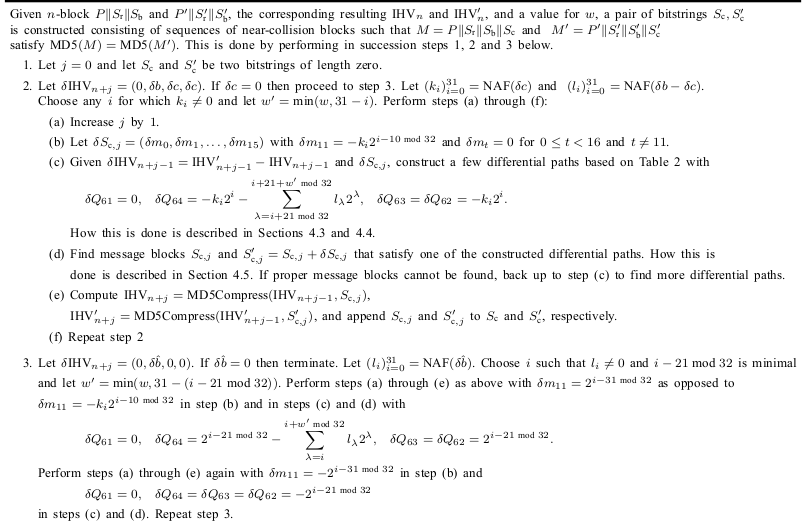
\includegraphics[scale=.61]{./pics/ncb.png}
  \caption{Algoritme de recherche des blocs de quasi-collisons}
\end{figure}

\begin{figure}
  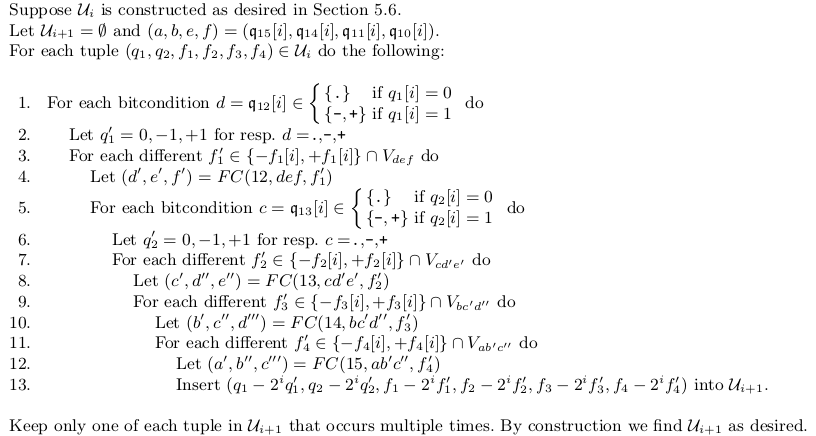
\includegraphics[scale=.61]{./pics/ui.png}
  \caption{Algorithme de construction du chemin différentiel}
\end{figure}


\newpage
\large{Bibliographie}
\bibliographystyle{style}
\bibliography{collision}


dopte 18565559

\end{document}